\chapter{Semantic Encoder Influence on G.U.}
\label{ch:semantic-encoder}


\section{Motivation} 

In their implementation of generative uncertainty, \parencite{jazbec_generative_2025} added a semantic encoder to avoid computing uncertainty in a pixel space that is overly sensitive to minor pixel-level details. 

\cite{jazbec_generative_2025} stated a theoretical gap to fill with regard to how this integrates into the Bayesian framework. 
Their conclusion was that the semantic encoder made the uncertainty measure possible, but they have not measured the role the approximated Bayesian framework played in their uncertainty metric. 

\section{Hypothesis}

This leaves the door open to the question: ``What if the semantic encoder actually contains most of the uncertainty evaluation capability?'' We hypothesize that uncertain images are very unstable in the semantic space: a slight change in an uncertain image leads to a large change in semantic space. We could therefore make random changes to the images and get a high uncertainty score if the starting image was already in an unstable region of the semantic encoder, making the Laplace Approximation unnecessary.

\section{Experiment}

\begin{figure}[!htbp]
    \centering
    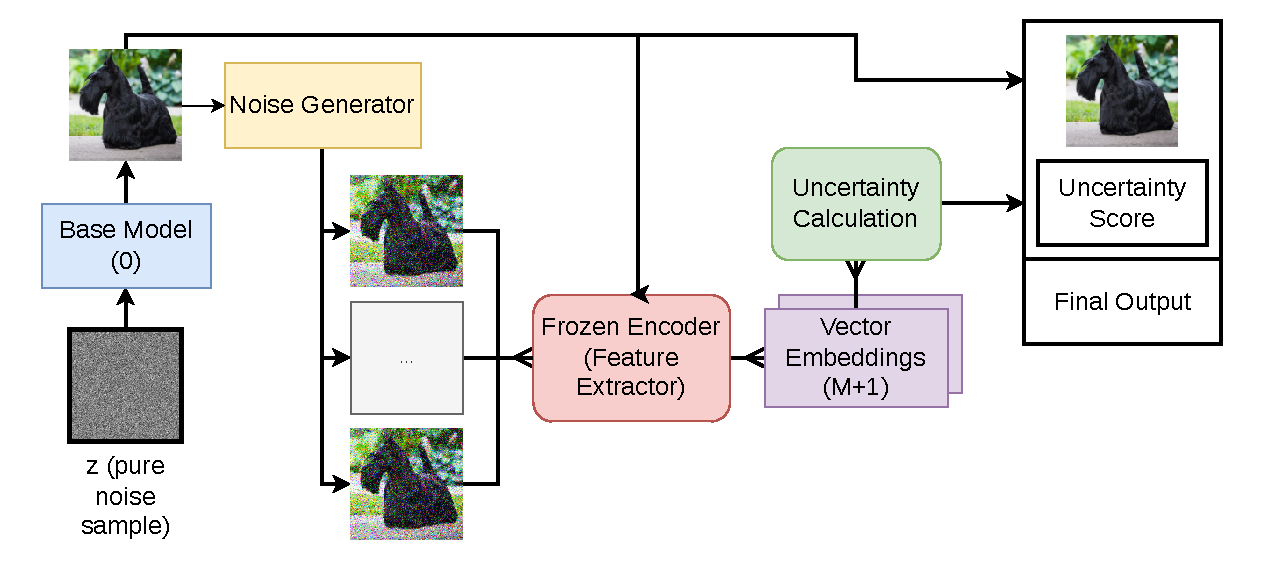
\includegraphics[width=0.8\linewidth]{figures/la_role/dni_pipeline.pdf}
    \caption{\acs{DNI} Pipeline (\warning the noise injected is exaggerated, in practice we use much less noise)}
    \label{fig:dni_pipeline}
\end{figure}

To test this hypothesis, we conduct an experiment where instead of using M models from the Laplace Approximated posterior distribution, we entirely skip the M models and use the generated image from the base model and add random noise to the image to create M additional images, we call this direct noise injection (\acs{DNI}). We can then use the same exact uncertainty score evaluation pipeline as before and measure how well it performs on the \acs{FPR} and \acs{HPS} metrics. The modified uncertainty calculation pipeline is illustrated on \autoref{fig:dni_pipeline}.

\section{Results Analysis}

\paragraph{HPSv3 Metric} On \autoref{fig:la_role_hps} we can barely differentiate the performance of the LLLA from the DNI (\acs{AURC}: \acs{LLLA} $= 12.84$ vs.\ \acs{DNI} $= 12.82$).

\begin{figure}[!htbp]
    \centering
    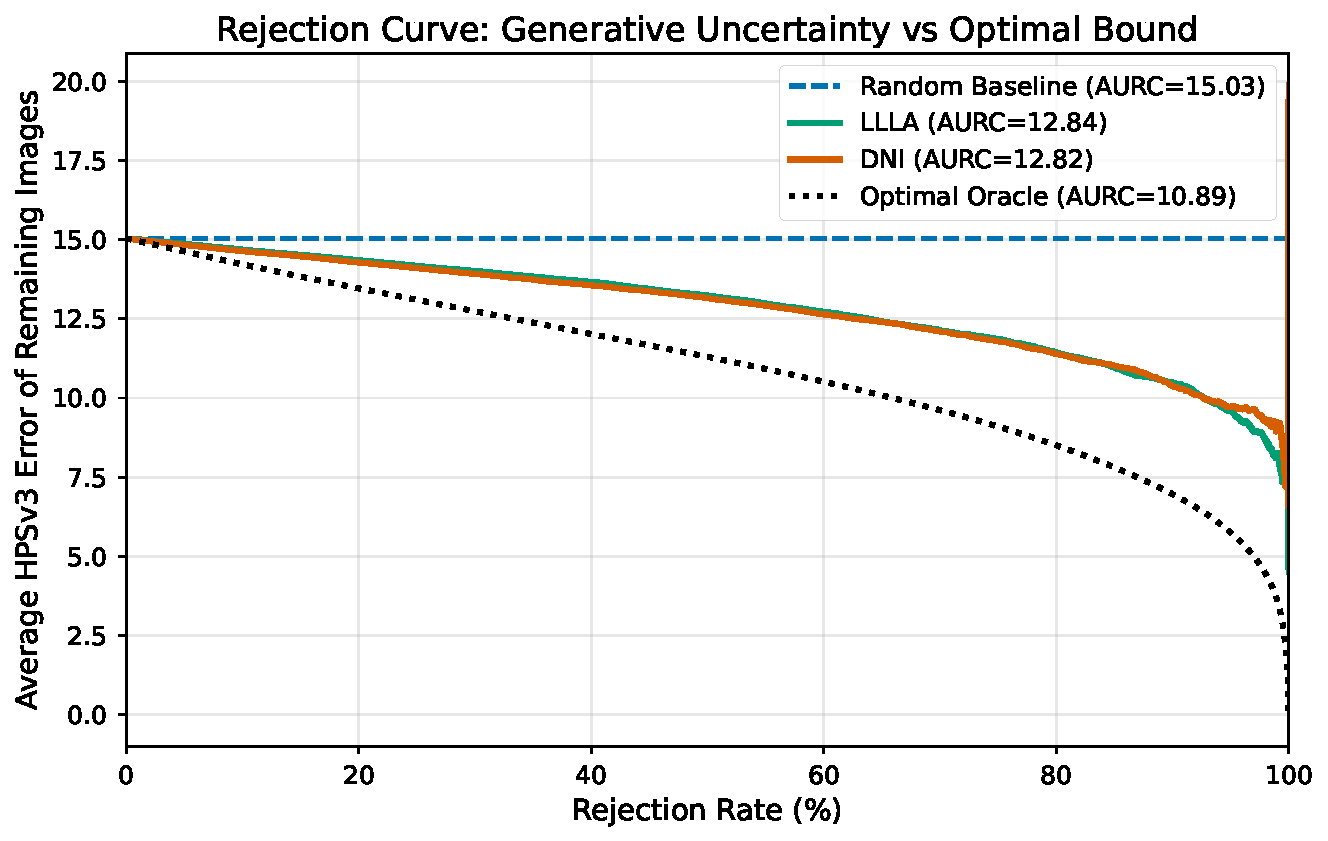
\includegraphics[width=0.7\linewidth]{figures/la_role/aurc_hps_llla_dni.pdf}
    \caption{Average HPSv3 error of the remaining images when filtering with either \acs{LLLA} or \acs{DNI} as a function of the percentage of rejected images}
    \label{fig:la_role_hps}
\end{figure}

\paragraph{FID, Precision and Recall} We almost get the same story on \autoref{fig:la_role_fpr} with a slight increase of \acs{FID} for the \acs{DNI} compared to the \acs{LLLA}.

\begin{figure}[!htbp]
    \centering
    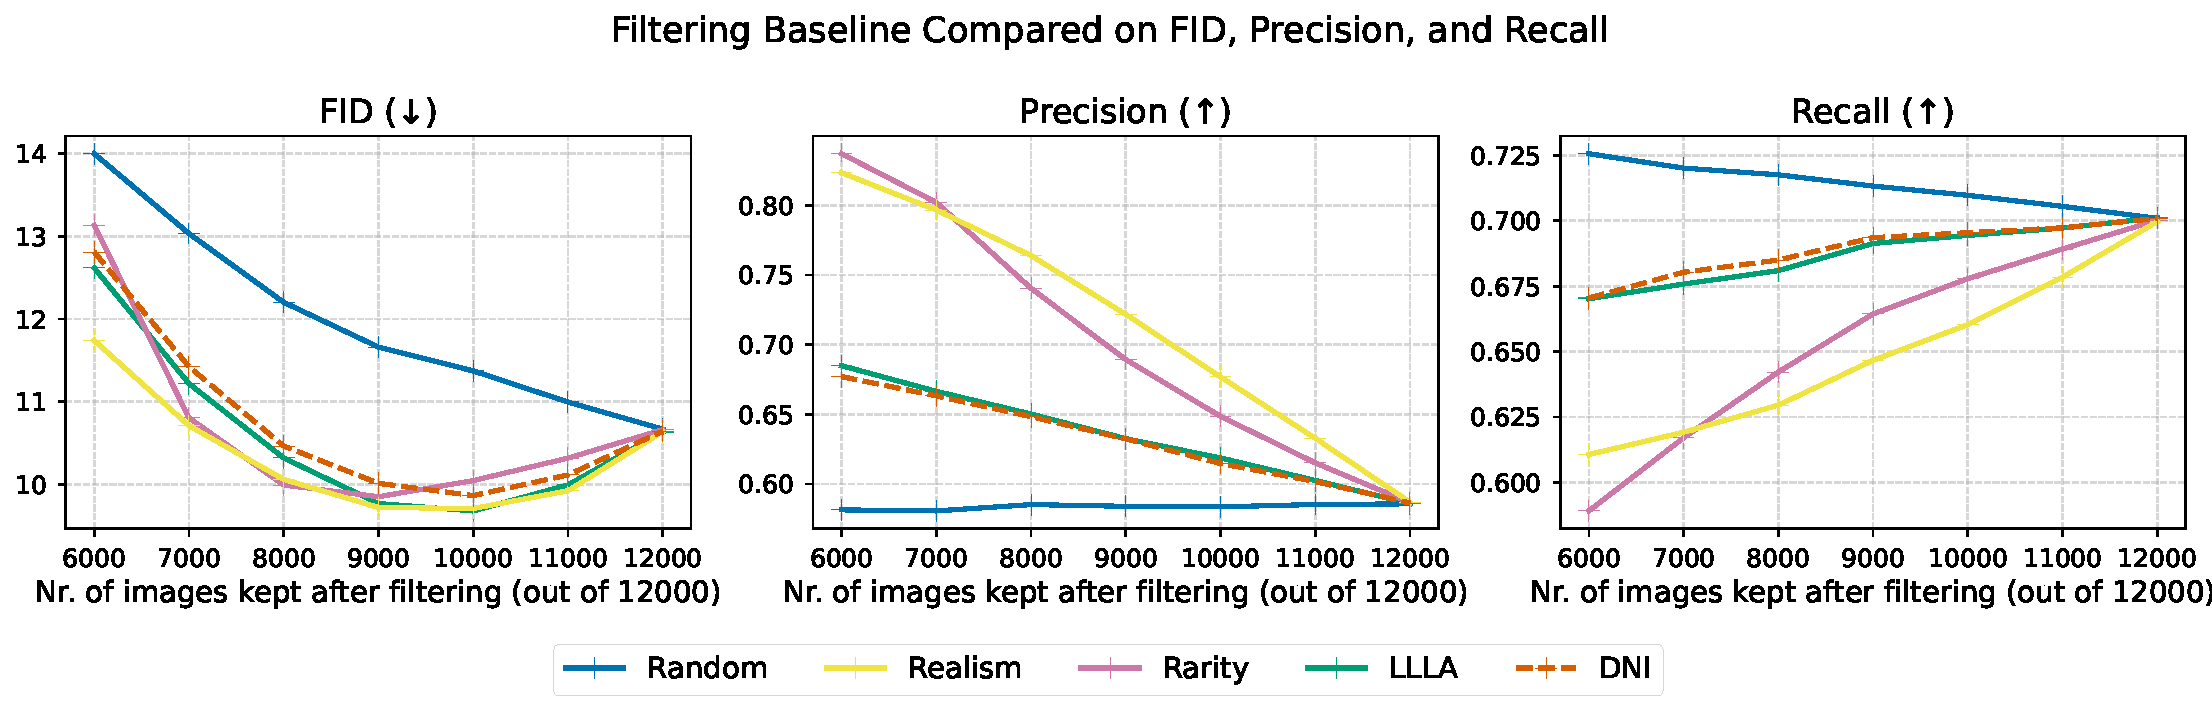
\includegraphics[width=0.99\linewidth]{figures/la_role/metrics_llla_dni.pdf}
    \caption{\cite{jazbec_generative_2025} \acs{FPR} Metrics to compare \acs{LLLA}, \acs{DNI}, (and Realism, Rarity)}
    \label{fig:la_role_fpr}
\end{figure}

\paragraph{Correlation}

The correlation plot \autoref{fig:la_role_corr} however shows that despite both methods achieving very similar performance on filtering out the dataset of 12032 images, they don't align perfectly (more on that in \autoref{sec:bayesian-model-over-approx}).

\begin{figure}[!htbp]
    \centering
    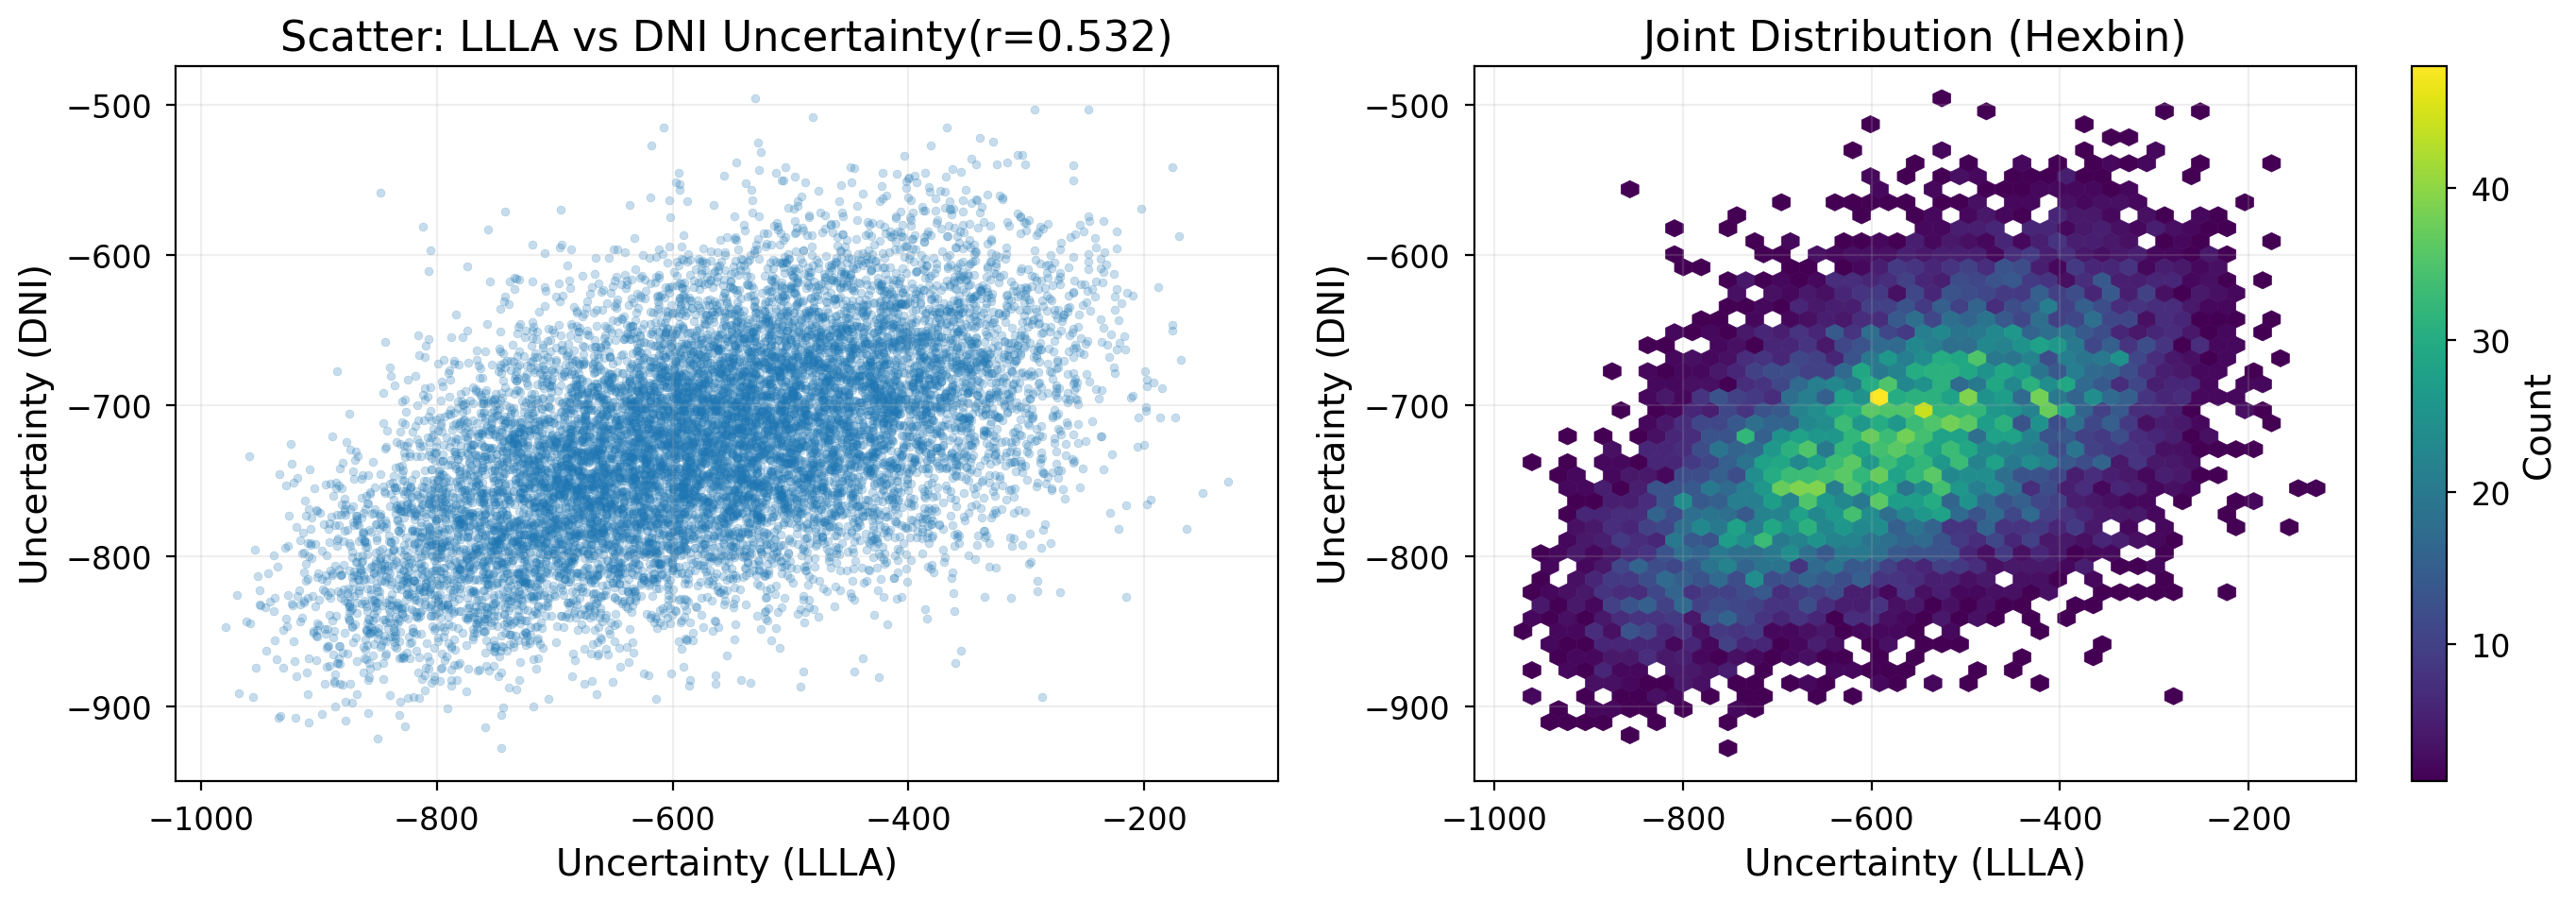
\includegraphics[width=0.8\linewidth]{figures/la_role/llla_dni_corr.png}
    \caption{Scatter plot and Density plot to show the correlation using LLLA uncertainty on the x-axis and DNI uncertainty on the y-axis. The Pearson correlation coefficient is $0.532$}
    \label{fig:la_role_corr}
\end{figure}

\section{Formalizing the Method}
\label{sec:formalize_dni_method}

How can such a simple method perform this close to the much more complex and expensive Laplace approximation method?

By bypassing the posterior entirely (\autoref{fig:dni_pipeline}), we completely departed from Bayesian theory here, we are not analyzing the model's knowledge but rather the encoder's confidence and proving that it's enough to filter out bad images.

We will now formalize the mathematical framework behind this method to explain its success.

\subsection{Formalizing the Post-Hoc Perturbation Framework}

Let $x \in \mathbb{R}^D$ be the output image generated by a the base model, and let $c_\phi: \mathbb{R}^D \rightarrow \mathbb{R}^K$ denote the semantic encoder (e.g., \acs{CLIP}) parameterized by $\phi$, which maps the high-dimensional pixel space into a $K$-dimensional semantic space. 

Instead of relying on the very expensive posterior predictive distribution of \parencite{jazbec_generative_2025}, we bypass the Bayesian framework entirely. We define a local pixel-space neighborhood around the final generated output $x$ of the base model by injecting isotropic Gaussian noise $\epsilon$:

\begin{align}
\tilde{x} = x + \epsilon \quad \text{where} \quad \epsilon \sim \mathcal{N}(0, \sigma_{noise}^2 I_D)
\end{align}

Following the evaluation protocol of \cite{jazbec_generative_2025}, we get the uncertainty of the original image $x$ by fitting a diagonal Gaussian distribution on the semantic embeddings $\tilde{e} = c_\phi(\tilde{x})$ and computing its entropy. 

Let $\sigma_{\tilde{e},i}^2$ be the variance of the $i$-th semantic dimension. The uncertainty $\mathcal{U}(x)$ is defined as the entropy of the diagonal Gaussian:

\begin{equation}
\mathcal{U}(x) = \frac{1}{2} \sum_{i=1}^K \ln(\sigma_{\tilde{e},i}^2) + const
\end{equation}

\begin{tcolorbox}[colback=orange!10!white,colframe=orange!50!black,sharp corners]
\warning here we are first working with $\tilde{e}$ as a random variable to show analytically the relationship between the uncertainty and the Jacobian of the encoder. To finalize the link with our experiment, we later prove that we can approximate the quantities associated to $\tilde{e}$ (such as the diagonal terms of its covariance matrix) with Monte Carlo.
\end{tcolorbox}

\subsection{The Jacobian Norm and Entropy Explosion}

To understand why this input-driven entropy $\mathcal{U}(x)$ acts as an effective proxy for generative quality, we analyze the local dynamics of the encoder $c_\phi$. For a sufficiently small noise variance $\sigma_{noise}^2$, the deviation in the semantic space can be approximated using a first-order Taylor expansion around $x$ (we denote this approximation as $\mathcal{T}$):

\begin{equation}
\tilde{e} = c_\phi(\tilde{x})= c_\phi(x + \epsilon) \overset{\mathcal{T}}{\approx} c_\phi(x) + J_\phi(x)\epsilon
\end{equation}

where $J_\phi(x) \in \mathbb{R}^{K \times D}$ is the Jacobian matrix of the encoder. 

The theoretical covariance of the resulting semantic embeddings $\Sigma_{\tilde{e}}$ is governed by the Jacobian:
\begin{align}
    \Sigma_{\tilde{e}} := \text{Cov}(\tilde{e}) &\overset{\mathcal{T}}{\simeq} \text{Cov}(\underbrace{c_{\phi}(x)}_{const} + J_{\phi}(x)\epsilon) \nonumber \\
    &= \text{Cov}(\underbrace{J_\phi(x)}_{const}\epsilon) \nonumber \\
    &= J_{\phi}(x)\text{Cov}(\epsilon)J_{\phi}(x)^{T} \nonumber \\
    &= J_\phi(x) (\sigma_{noise}^2 I_D) J_\phi(x)^T \nonumber \\
    &= \sigma_{noise}^2 J_\phi(x) J_\phi(x)^T
\end{align}

Because we are fitting a diagonal Gaussian, we are specifically interested in the diagonal elements of $\Sigma_{\tilde{e}}$.
% which are linked to our empirical variances $\hat{\sigma}_{\tilde{e},i}^2$. 
Mathematically, the $i$-th diagonal element of this matrix is the squared $L_2$ norm of the $i$-th row of the Jacobian:

\begin{equation}
\sigma_{\tilde{e},i}^2 \overset{\mathcal{T}}{\simeq} \sigma_{noise}^2 \|\nabla c_{\phi, i}(x)\|_2^2
\end{equation}

Substituting this into our entropy formulation reveals the direct theoretical link:

\begin{equation}
\mathcal{U}(x) \overset{\mathcal{T}}{\simeq} \frac{1}{2} \sum_{i=1}^K \ln\left( \sigma_{noise}^2 \|\nabla c_{\phi, i}(x)\|_2^2 \right) + const \label{eq:jacobian_uncertainty}
\end{equation}


\subsection{Monte Carlo Approximation}

The missing link to match our experiment to this mathematical framework is the Monte Carlo approximation of the variance terms $\sigma^2_{\tilde{e},i}$ by going from the random variable space $\tilde{x}$ to a fixed number of samples $\tilde{x}_m$ $m \in \{0,\dots,M\}$ (With $x_0$ the base model output and $x_{m\leq1}$ the noise perturbed samples). We can approximate those terms as follows:

\begin{align}
\sigma_{\tilde{e},i}^2 \simeq \frac{1}{M-1} \sum_{m=0}^{M} (\tilde{e}_{m,i} - \bar{e}_i)^2
\end{align}

Where $\bar{e}_i = \frac{1}{M} \sum^M_{m=0} \tilde{e}_{m,i}$

We can finally say \autoref{eq:jacobian_uncertainty} proves that the entropy score we extract from the perturbed ensemble is intrinsically driven by the logarithmic sum of the squared gradients (the localized Jacobian norms) of the semantic encoder. We see next why this is important.

\subsection{Generative Failure as Off-Manifold Instability}

The connection to the Jacobian dictates our capability to detect generative failures. Let $\mathcal{M} \subset \mathbb{R}^D$ represent the low-dimensional data manifold of natural images learned during the encoder's training.

If a diffusion model then generates a high-quality, confident image $x$, it is highly likely that this image lives in $\mathcal{M}$ where the local Lipschitz constant of $c_\phi$ is small \parencite{novak_sensitivity_2018}. The gradients $\|\nabla c_{\phi, i}(x)\|_2^2$ are bounded by a small value, resulting in small variances $\sigma_{\tilde{e},i}^2$, and consequently, a low, stable entropy $\mathcal{U}(x)$.

Conversely, if the generative model fails and produces an image with severe structural artifacts, the sample falls out-of-distribution ($x \notin \mathcal{M}$). In these off-manifold regions, the encoder becomes highly non-linear and sensitive \cite{novak_sensitivity_2018}, causing the local gradient norms $\|\nabla c_{\phi, i}(x)\|_2^2$ to explode. Because our formulation shows that the dimensional variance $\sigma_{\tilde{e},i}^2$ scales directly with these exploding gradients, the resulting entropy $\mathcal{U}(x)$ undergoes a massive increase.

Therefore, estimating entropy via post-hoc pixel perturbations successfully isolates the exact same off-manifold instability as complex weight-space posteriors, justifying its competitive performance.

This perturbation-and-variance recipe is not itself new. It mirrors test-time augmentation (\acs{TTA}), where inputs are perturbed at inference and the spread of the resulting predictions is read as an uncertainty estimate \parencite{wang_aleatoric_2019}, and it is close in spirit to \cite{vita_diffusion_2024}, who filter diffusion samples using the variance of the denoising scores under perturbation. \cite{jazbec_generative_2025} however tested the Aleatoric Uncertainty method of \cite{vita_diffusion_2024} and found it to be ineffective on the \acs{FPR} metrics.

\section{Bayesian Model Over-Approximation}
\label{sec:bayesian-model-over-approx}

\paragraph{Bayesian Approximation Rendered to Noise}
Before concluding on this experiment, we should be reminded that the Bayesian method used here and in \cite{jazbec_generative_2025} is heavily approximated, which certainly reduced the uncertainty signal strength coming out of the diffusion model, and it might have been to the point where that uncertainty signal essentially became noise that was fed through the encoder the same way \acs{DNI} does it. 

The correlation plot and Pearson coefficient $r=0.532$ (\autoref{fig:la_role_corr}) give a nuanced picture: it shows that the uncertainty might not have become fully random noise, otherwise we could expect a stronger correlation. But since both \acs{DNI} and \acs{LLLA} perform almost identically on \acs{FPR} and \acs{HPS} metrics, the difference in scores observed on the correlation plot could also be attributed to uncertainty inherent to the calculation of ``generative uncertainty'' through an external encoder with a limited number of samples ($\mathrm{M}+1$). That per-sample score uncertainty would be averaged out when taking the batch-scale metrics.

\paragraph{Bayesian Uncertainty is Valuable}
It is possible that a proper, more accurate Bayesian approximation, akin to what \cite{gegenfurtner_reducing_2026} did, would provide an uncertainty signal strong enough to go through the encoder and still provide value.

But we might not even need a more accurate Bayesian approximation. In the context of a Toy model that outputs in 2D space and therefore doesn't need a semantic encoder, we show in \autoref{ch:toy_exp_posterior} that a simple \acs{LLLA} can already provide a very strong uncertainty signal that is enough to filter out OOD samples. The only difference between the \acs{ADM} \acs{LLLA} and the \textit{Toy Model} \acs{LLLA} for the posterior is that the former uses only 1\% of the training data to compute the approximation while the latter uses the full training set (\autoref{sub:gu_th_toy_model_posterior_approximation}). The problem with the current \acs{ADM} \acs{LLLA} could be that 1\% is not enough or that the \acs{LLLA} is too simple for the complexity of the \acs{ADM} compared to the significantly simpler \textit{Toy Model} or other reasons that all need further investigation as future work.

% But in the context of the \textit{Toy Model} (\autoref{ch:toy_exp_posterior}) we prove that the \acs{LLLA} by itself (without a semantic encoder) is highly effective at filtering out \acs{OOD} samples provided we done a proper regularization and scaling of that posterior approximation.

% The only difference between the \acs{ADM} \acs{LLLA} and \textit{Toy Model} \acs{LLLA} is the 


\section{Conclusion}

We've shown that \acs{DNI} gets very close to the results of \cite{jazbec_generative_2025}, and the formalization and prior-work discussion above explain why: a known perturbation-and-variance mechanism, applied through the encoder, suffices.

We can however no longer talk about Generative Uncertainty with a method that bypasses the whole Bayesian framework and does not care about the generative model itself. 

Regardless of whether the heavily approximated Bayesian framework provides any value compared to simply using random noise, using an external encoder trained on a different dataset than the one used to train the actual diffusion model does not make sense when we want to properly isolate the uncertainty of the diffusion model itself.
The \acs{ADM} needs an alternative to the external semantic encoder to allow for an uncontaminated measurement of its uncertainty and we explore this in the next chapter (\autoref{ch:using_internal_encoder}).